% В этом файле следует писать текст работы, разбивая его на
% разделы (section), подразделы (subsection) и, если нужно,
% главы (chapter).

% Предварительно следует указать необходимую информацию
% в файле SETUP.tex

%% В этот файл не предполагается вносить изменения

% В этом файле следует указать информацию о себе
% и выполняемой работе.

\documentclass [fontsize=14pt, paper=a4, pagesize, DIV=calc]%
{scrreprt}
% ВНИМАНИЕ! Для использования глав поменять
% scrartcl на scrreprt

% Здесь ничего не менять
\usepackage [T2A] {fontenc}   % Кириллица в PDF файле
\usepackage [utf8] {inputenc} % Кодировка текста: utf-8
\usepackage [russian] {babel} % Переносы, лигатуры

%%%%%%%%%%%%%%%%%%%%%%%%%%%%%%%%%%%%%%%%%%%%%%%%%%%%%%%%%%%%%%%%%%%%%%%%
% Создание макроса управления элементами, специфичными
% для вида работы (курс., бак., маг.)
% Здесь ничего не менять:
\usepackage{ifthen}
\newcounter{worktype}
\newcommand{\typeOfWork}[1]
{
	\setcounter{worktype}{#1}
}

% ВНИМАНИЕ!
% Укажите тип работы: 0 - курсовая, 1 - бак., 2 - маг.,
% 3 - бакалаврская с главами.
\typeOfWork{2}
% Считается, что курсовая и бак. бьются на разделы (section) и
% подразделы (subsection), а маг. — на главы (chapter), разделы и
%  подразделы. Если хочется,
% чтобы бак. была с главами (например, если она большая),
% надо выбрать опцию 3.

% Если при выборе 2 или 3 вы забудете поменять класс
% документа на scrreprt (см. выше, в самом начале),
% то получите ошибку:
% ./aux/appearance.tex:52: Package scrbase Error: unknown option ` chapterprefix=

%%%%%%%%%%%%%%%%%%%%%%%%%%%%%%%%%%%%%%%%%%%%%%%%%%%%%%%%%%%%%%%%%%%%%%%%
% Информация об авторе и работе для титульной страницы

\usepackage {titling}

% Имя автора в именительном падеже (для маг.)
\newcommand {\me}{%
G.\,A.~Lukyanov%
}

% Имя автора в родительном падеже (для курсовой и бак.)
\newcommand {\byme}{%
И.\,И.~Иванова%
}

% Любимый научный руководитель
\newcommand{\supervisor}%
{учёная степень, учёное звание /  должность И. О. Фамилия}

% идентифицируем пол (только для курсовой и бак.)
\newcommand{\bystudent}{
Студента %Студентки % Для курсовой: с большой буквы
}

% Год публикации
\date{2017}

% Название работы
\title{Constructing effectful computations}

% Кафедра
%
\newboolean{needchair}
\setboolean{needchair}{false} % на ФИИТ не пишется (false), на ПМИ есть (true)

\newcommand {\thechair} {%
Кафедра компьютерного и аналогового моделирования светлого будущего%
}

\newcommand {\direction} {%
Направление подготовки\\
Фундаментальная информатика и информационные технологии%
}% Прикладная математика и информатика

%%%%%%%%%%%%%%%%%%%%%%%%%%%%%%%%%%%%%%%%%%%%%%%%%%%%%%%%%%%%%%%%%%%%%%%%
% Другие настраиваемые элементы текста

% Листинги с исходным кодом программ: укажите язык программирования
\usepackage{listings}
\lstset{
    language=Haskell,%  Язык указать здесь
    basicstyle=\small\ttfamily,
    breaklines=true,%
    showstringspaces=false%
    inputencoding=utf8x%
}
% полный список языков, поддерживаемых данным пакетом, есть,
% например, здесь (стр. 13):
% ftp://ftp.tex.ac.uk/tex-archive/macros/latex/contrib/listings/listings.pdf

% Нумерация списков: можно при необходимести
% изменять вид нумерации (например, добавлять правую скобку).
% По умолчанию буду списки вида:
% 1.
% 2.
% Изменять вид нумерации можно в начале нумерации:
% \begin{enumerate}[1)] (В квадратных скобках указан желаемый вид)
\usepackage[shortlabels]{enumitem}
                    \setlist[enumerate, 1]{1.}

% Гиперссылки: настройте внешний вид ссылок
\usepackage%
[pdftex,unicode,pdfborder={0 0 0},draft=false,%backref=page,
    hidelinks, % убрать, если хочется видеть ссылки: это
               % удобно в PDF файле, но не должно появиться на печати
    bookmarks=true,bookmarksnumbered=false,bookmarksopen=false]%
{hyperref}


\usepackage {amsmath}      % Больше математики
\usepackage {amssymb}
\usepackage {textcase}     % Преобразование к верхнему регистру
\usepackage {indentfirst}  % Красная строка первого абзаца в разделе
\usepackage [super]{nth}

\usepackage {fancyvrb}     % Листинги: определяем своё окружение Verb
\DefineVerbatimEnvironment% с уменьшенным шрифтом
	{Verb}{Verbatim}
	{fontsize=\small}

% Вставка рисунков
\usepackage {graphicx}

% Общее оформление
% ----------------------------------------------------------------
% Настройка внешнего вида

%%% Шрифты

% если закомментировать всё — консервативная гарнитура Computer Modern
\usepackage{paratype} % профессиональные свободные шрифты
%\usepackage {droid}  % неплохие свободные шрифты от Google
%\usepackage{mathptmx}
%\usepackage {mmasym}
%\usepackage {psfonts}
%\usepackage{lmodern}
%var1: lh additions for bold concrete fonts
%\usepackage{lh-t2axccr}
%var2: the package below could be covered with fd-files
%\usepackage{lh-t2accr}
%\usepackage {pscyr}

% Геометрия текста

\usepackage{setspace}       % Межстрочный интервал
\onehalfspacing

\newlength\MyIndent
\setlength\MyIndent{1.25cm}
\setlength{\parindent}{\MyIndent} % Абзацный отступ
\frenchspacing            % Отключение лишних отступов после точек
\KOMAoptions{%
    DIV=calc,         % Пересчёт геометрии
    numbers=endperiod % точки после номеров разделов
}

                            % Консервативный вариант:
%\usepackage                % ручное задание геометрии
%[%                         % (не рекомендуется в проф. типографии)
%  margin = 2.5cm,
  %includefoot,
  %footskip = 1cm
%] %
%  {geometry}

%%% Заголовки

\ifthenelse{\equal{\theworktype}{2}}{%
\KOMAoptions{%
    numbers=endperiod,% точки после номеров разделов
    headings=normal,   % размеры заголовков поменьше стандартных
    chapterprefix=true,% Печатать слово Глава в магистерской
    appendixprefix=true% Печатать слово Приложение
}
}

% шрифт для оформления глав и названия содержания
\newcommand{\SuperFont}{\Large\sffamily\bfseries}

% Заголовок главы
\ifthenelse{\value{worktype} > 1}{%
\renewcommand{\SuperFont}{\Large\normalfont\sffamily}
\newcommand{\CentSuperFont}{\centering\SuperFont}
\usepackage{fncychap}
\ChNameVar{\SuperFont}
\ChNumVar{\CentSuperFont}
\ChTitleVar{\CentSuperFont}
\ChNameUpperCase
\ChTitleUpperCase
}

% Заголовок (под)раздела с абзацного отступа
\addtokomafont{sectioning}{\hspace{\MyIndent}}

\renewcommand*{\captionformat}{~---~}
\renewcommand*{\figureformat}{Listing~\thefigure}

% Плавающие листинги
\usepackage{float}
\floatstyle{ruled}
\floatname{ListingEnv}{Листинг}
\newfloat{ListingEnv}{htbp}{lol}[section]

% точка после номера листинга
\makeatletter
\renewcommand\floatc@ruled[2]{{\@fs@cfont #1.} #2\par}
\makeatother


%%% Оглавление
\usepackage{tocloft}

% шрифт и положение заголовка
\ifthenelse{\value{worktype} > 1}{%
\renewcommand{\cfttoctitlefont}{\hfil\SuperFont\MakeUppercase}
}{
\renewcommand{\cfttoctitlefont}{\hfil\SuperFont}
}

% слово Глава
\usepackage{calc}
\ifthenelse{\value{worktype} > 1}{%
\renewcommand{\cftchappresnum}{Chapter }
\addtolength{\cftchapnumwidth}{\widthof{Chapter }}
}

\newcommand{\setupname}[1]{%
  \addtocontents{toc}{%
    \unexpanded{\unexpanded{%
      \renewcommand{\cftchappresnum}{#1 }%
      \setlength\cftchapnumwidth{\widthof{\bfseries #1 }}%
      \addtolength\cftchapnumwidth{\fixedchapnumwidth}%
    }}%
  }%
}
\AtBeginDocument{\edef\fixedchapnumwidth{\the\cftchapnumwidth}}

% Очищаем оформление названий старших элементов в оглавлении
\ifthenelse{\value{worktype} > 1}{%
\renewcommand{\cftchapfont}{}
\renewcommand{\cftchappagefont}{}
}{
\renewcommand{\cftsecfont}{}
\renewcommand{\cftsecpagefont}{}
}

% Точки после верхних элементов оглавления
\renewcommand{\cftsecdotsep}{\cftdotsep}
%\newcommand{\cftchapdotsep}{\cftdotsep}

\ifthenelse{\value{worktype} > 1}{%
    \renewcommand{\cftchapaftersnum}{.}
}{}
\renewcommand{\cftsecaftersnum}{.}
\renewcommand{\cftsubsecaftersnum}{.}
\renewcommand{\cftsubsubsecaftersnum}{.}

%%% Списки (enumitem)

\usepackage {enumitem}      % Списки с настройкой отступов
\setlist %
{ %
  leftmargin = \parindent, itemsep=.5ex, topsep=.4ex
} %

% По ГОСТу нумерация должны быть буквами: а, б...
%\makeatletter
%    \AddEnumerateCounter{\asbuk}{\@asbuk}{м)}
%\makeatother
%\renewcommand{\labelenumi}{\asbuk{enumi})}
%\renewcommand{\labelenumii}{\arabic{enumii})}

%%% Таблицы: выбрать более подходящие

\usepackage{booktabs} % считаются наиболее профессионально выполненными
%\usepackage{ltablex}
%\newcolumntype {L} {>{---}l}

%%% Библиография

\usepackage{csquotes}        % Оформление списка литературы
\usepackage[
  backend=biber,
  hyperref=auto,
  sorting=none, % сортировка в порядке встречаемости ссылок
  language=auto,
  citestyle=gost-numeric,
  bibstyle=gost-numeric
]{biblatex}
\addbibresource{biblio.bib} % Файл с лит.источниками

% Настройка величины отступа в списке
\ifthenelse{\value{worktype} < 2}{%
\defbibenvironment{bibliography}
  {\list
     {\printtext[labelnumberwidth]{%
    \printfield{prefixnumber}%
    \printfield{labelnumber}}}
     {\setlength{\labelwidth}{\labelnumberwidth}%
      \setlength{\leftmargin}{\labelwidth}%
      \setlength{\labelsep}{\dimexpr\MyIndent-\labelwidth\relax}% <----- default is \biblabelsep
      \addtolength{\leftmargin}{\labelsep}%
      \setlength{\itemsep}{\bibitemsep}%
      \setlength{\parsep}{\bibparsep}}%
      \renewcommand*{\makelabel}[1]{\hss##1}}
  {\endlist}
  {\item}
}{}

% ----------------------------------------------------------------
% Настройка переносов и разрывов страниц

\binoppenalty = 10000      % Запрет переносов строк в формулах
\relpenalty = 10000        %

\sloppy                    % Не выходить за границы бокса
%\tolerance = 400          % или более точно
\clubpenalty = 10000       % Запрет разрывов страниц после первой
\widowpenalty = 10000      % и перед предпоследней строкой абзаца

% ----------------------------


% Стили для окружений типа Определение, Теорема...
% Оформление теорем (ntheorem)

\usepackage [thmmarks, amsmath] {ntheorem}
\theorempreskipamount 0.6cm

\theoremstyle {plain} %
\theoremheaderfont {\normalfont \bfseries} %
\theorembodyfont {\slshape} %
\theoremsymbol {\ensuremath {_\Box}} %
\theoremseparator {:} %
\newtheorem {mystatement} {Утверждение} [section] %
\newtheorem {mylemma} {Лемма} [section] %
\newtheorem {mycorollary} {Следствие} [section] %

\theoremstyle {nonumberplain} %
\theoremseparator {.} %
\theoremsymbol {\ensuremath {_\diamondsuit}} %
\newtheorem {mydefinition} {Определение} %

\theoremstyle {plain} %
\theoremheaderfont {\normalfont \bfseries} 
\theorembodyfont {\normalfont} 
%\theoremsymbol {\ensuremath {_\Box}} %
\theoremseparator {.} %
\newtheorem {mytask} {Задача} [section]%
\renewcommand{\themytask}{\arabic{mytask}}

\theoremheaderfont {\scshape} %
\theorembodyfont {\upshape} %
\theoremstyle {nonumberplain} %
\theoremseparator {} %
\theoremsymbol {\rule {1ex} {1ex}} %
\newtheorem {myproof} {Доказательство} %

\theorembodyfont {\upshape} %
%\theoremindent 0.5cm
\theoremstyle {nonumberbreak} \theoremseparator {\\} %
\theoremsymbol {\ensuremath {\ast}} %
\newtheorem {myexample} {Пример} %
\newtheorem {myexamples} {Примеры} %

\theoremheaderfont {\itshape} %
\theorembodyfont {\upshape} %
\theoremstyle {nonumberplain} %
\theoremseparator {:} %
\theoremsymbol {\ensuremath {_\triangle}} %
\newtheorem {myremark} {Замечание} %
\theoremstyle {nonumberbreak} %
\newtheorem {myremarks} {Замечания} %


% Титульный лист
% Макросы настройки титульной страницы
% В этот файл не предполагается вносить изменения

%\usepackage {showframe}

% Вертикальные отступы на титульной странице
\newcommand{\vgap}{\vspace{16pt}}

% Помещение города и даты в нижний колонтитул
\usepackage{scrlayer}
\DeclareNewLayer[
  foot,
  foreground,
  contents={%
    \raisebox{\dp\strutbox}[\layerheight][0pt]{%
      \parbox[b]{\layerwidth}{\centering Ростов-на-Дону\\ \thedate%
       \\\mbox{}
       }}%
  }
]{titlepage.foot.fg}
\DeclareNewPageStyleByLayers{titlepage}{titlepage.foot.fg}


\AtBeginDocument %
{ %
  %
  \begin{titlepage}
  %
    \thispagestyle{titlepage}

    {\centering
    %
    \MakeTextUppercase {МИНИСТЕРСТВО ОБРАЗОВАНИЯ И НАУКИ РФ}

    \vgap

    Федеральное государственное автономное образовательное\\
    учреждение высшего образования\\
    \MakeTextUppercase {Южный федеральный университет}

    \vgap

	Институт математики, механики и компьютерных наук
    имени~И.\,И.\,Воровича

    \vgap

    \direction

    \ifthenelse{\boolean{needchair}}{
    \vgap

    \thechair}{}

    \vspace* {\fill}

    \ifthenelse{\value{worktype} = 2}{%
    \me

    \vgap}{}

    {\usefont{T2A}{PTSansCaption-TLF}{m}{n}
    \MakeTextUppercase{\thetitle}}

    \ifthenelse{\value{worktype} = 2}{%
     \vgap

    Магистерская диссертация}{}
    \ifthenelse{\value{worktype} = 0}{
     \vgap

    Курсовая работа
    }{}%
    \ifthenelse{\value{worktype} = 1 \OR \value{worktype} = 3}{
     \vgap

    Выпускная квалификационная работа\\
    на степень бакалавра
    }{}%

    \vspace {\fill}

    \begin{flushright}
    \ifthenelse{\value{worktype} = 0 \OR
                \value{worktype} = 1 \OR
                \value{worktype} = 3}{
      \bystudent \ifthenelse{\value{worktype} = 0}{3}{4}\ курса\\
      \byme
    }{}

    \vgap

    Научный руководитель:\\
    к.т.н., с.н.с., доц. каф. ИВЭ
    А.~Н.~Литвиненко\\
    \ifthenelse{\value{worktype} = 2}{%
    Рецензент:\\
    к.ф.-м.н., доц., доц. каф. АДМ С.~С.~Михалкович}{}
	\end{flushright}
    \ifthenelse{\value{worktype} = 0}{
    \vspace{\fill}
            \begin{flushleft}
              \begin{tabular}{cc}
                \underline{\hspace{4cm}}&\underline{\hspace{5cm}}\\
                {\small оценка (рейтинг)} & {\small  подпись руководителя}\\
              \end{tabular}
            \end{flushleft}
    }{}
  	\vspace {\fill}
  %Ростов-на-Дону

    %\thedate

  }\end{titlepage}
  %
  %
  \tableofcontents
  %
  \clearpage
} %



% Команды для использования в тексте работы


% макросы для начала введения и заключения
\newcommand{\Ackns}{\addchap{Acknowledgements}}

\newcommand{\Intro}{\addchap{Introduction}}

\newcommand{\Goal}{\addchap{Goal statement}}

\newcommand{\Conc}{\addchap{Conclusion}}

% Правильные значки для нестрогих неравенств и пустого множества
\renewcommand {\le} {\leqslant}
\renewcommand {\ge} {\geqslant}
\renewcommand {\emptyset} {\varnothing}

% N ажурное: натуральные числа
\newcommand {\N} {\ensuremath{\mathbb N}}

% значок С++ — используйте команду \cpp
\newcommand{\cpp}{%
C\nolinebreak\hspace{-.05em}%
\raisebox{.2ex}{+}\nolinebreak\hspace{-.10em}%
\raisebox{.2ex}{+}%
}

% значок С# — используйте команду \cs
\newcommand{\cs}{%
C\nolinebreak\hspace{-.05em}%
\raisebox{.2ex}{\#}%
}

% Неразрывный дефис, который допускает перенос внутри слов,
% типа жёлто-синий: нужно писать жёлто"/синий.
\makeatletter
  \defineshorthand[english]{"/}{\babelhyphen{nobreak}}
  \addto\extrasenglish{
    \languageshorthands{english}
    \useshorthands{"}
  }
\makeatother



\endinput

% Конец файла


\begin{document}

Software systems are required to be reliable. For example, biomedical implants must be able to operate autonomously within patients, adapting to short term and long term changes, with required lifetimes in the order of decades, and one-minute downtime failure of banking software may lead to significant expenses. Safety and solidity of software may be achieved through testing and post-design quality assurance, but there is always a possibility to leave some branches of an operations scenario untested, leading to potential disaster.

In contrast with post-design testing, that doesn’t provide full
correctness guarantees, formal methods provide a systematic approach for developing complex systems in a correct by construction manner. One reason of advancement of
formal methods in comparison to testing is a maximal possible elimination of human errors. For instance, techniques known as model checking perform exhaustive search
through entire space of possible states of the system and evaluating system status in
every single state, completely excluding any possibility of non-specified behaviour (
presuming the correctness of specification).

One class of formal methods is advanced type systems provided by modern programming languages. Powerful yet lightweight formal verification techniques, provided by these languages are based on famous Curry-Howard correspondence --- a direct relationship between computer programs and mathematical
proofs --- that was discovered by the American mathematician Haskell Curry and logician
William Alvin Howard in late 1960s. A perfectly written Philip Wadler’s paper,
called ``Propositions as Types''~\cite{Wadler:2015:PT:2847579.2699407}
contains a great set of historical notes alongside with points of view on
Curry-Howard correspondence from different fields of
mathematics and computer science. Curry-Howard correspondence is of great value
for software developers because it provides a possibility to formulate desired
properties of programs in terms of types and automatically acquire proofs of
the correctness of those programs through type checking.

Advances in type theory and theory of programming languages led to the development and spreading of effects systems --- a particular kind of type-guided verification providing a possibility to separate pure computations from ones flavoured with a computational side effect, life, for instance, file system IO. These technique
was first given an account by Moggi~\cite{Moggi:1991:NCM:116981.116984} who
used monads to provide a denotational semantics to lambda calculus with effects, and then Wadler~\cite{Wadler:1992:EFP:143165.143169} gave monads a practical instantiation in Haskell programming language.

Computational effects control techniques got plenty of attention both in academic and software engineering communities. As applications, such as, for example, parsers combinators~\cite{monParsing} were explored, a lot more requirements and demands
were introduced: combine effects in a modular way, provide finer-grained control
for effects. This led to development of both monadic~\cite{Liang:1995:MTM:199448.199528} and alternative approaches~\cite{Mcbride:2008:APE:1348940.1348941}
~\cite{DBLP:journals/jlp/BauerP15}.

This work aims to research and development of programming languages features supporting explicit and precise control of computational effects. It addresses the problem
of construction of parser combinators libraries using three approaches to
effectful programming:

\begin{itemize}
  \item Monad transformers~\cite{Liang:1995:MTM:199448.199528} in~\texttt{Haskell}.
  \item Algebraic effects and effects handlers in a form of extensible.
  effects~\cite{Kiselyov:2013:EEA:2578854.2503791} in~\texttt{Haskell}
  \item~\texttt{Frank}~\cite{DBLP:conf/popl/LindleyMM17} programming language featuring first-class support of algebraic
  effects and effects handlers.
\end{itemize}

Main results of this work were presented in \nth{4} international conference ``Tools and Methods of Program Analysis 2017''~\cite{tmpa} in Moscow and conference
``Programming languages and compilers 2017'' in Rostov-on-Don.
Tell about scopus and ВАК publications.

Tell about structure of this thesis.



\chapter{Functional programming and computational effects}
~\label{cpt-effects}

Recent advances in theory of programming languages led to development and spreading
of functional programming languages with advanced type systems. This provide
software engineers a possibility to encode system specification in type-level, enforcing
statically checked guaranties of correctness. A large cluster of errors is
introduced into programs by uncontrolled side effects such as file system IO,
network communication and mutable state. When many mainstream programming languages such as \cpp,
Java and \cs~follow static type discipline, they do not track
side-effects, thus making it harder to reason about program correctness. In contrast,
pure languages like Haskell and Idris forbid programs to execute effectful code
without special type annotations.

\begin{figure}[h]
\begin {lstlisting}
int plus(int x, int y) {
  print("I'm mutating the World without you noticing!");
  return x + y;
}
\end{lstlisting}
\caption{Uncontrollable side-effect in an impure language}
\label{listing:effectfulPlus}
\end{figure}

\begin{figure}[h]
\begin{lstlisting}
plus :: Int -> Int -> Int
plut x y = x + y
\end{lstlisting}
\caption{Pure Haskell function}
\label{listing:purePlusHaskell}
\end{figure}

\begin{figure}[h]
\begin{lstlisting}
plusIO :: Int -> Int -> IO Int
plutIO x y = do
print "I'm mutating the World, but you know it"
return (x + y)
\end{lstlisting}
\caption{Pure Haskell function}
\label{listing:purePlusHaskell}
\end{figure}

After initial incorporation of side-effect control techniques in Haskell in
form of Monads~\cite{Wadler:1992:EFP:143165.143169}, effects systems got a lot
of development. Monadic approach has been enriched with the concept of monad
transformers~\cite{Liang:1995:MTM:199448.199528} to provide a modular way of
expressing computations with multiple side-effects. Even though monad
transformers has been widely accepted as a modular approach to side effects control,
they have some major drawbacks which are addressed, for instance, by Kiselyov at al.~\cite{Kiselyov:2013:EEA:2578854.2503791}, and alternative approach --- Algebraic effects and effects handlers --- was proposed~\cite{DBLP:journals/jlp/BauerP15}
~\cite{Kiselyov:2013:EEA:2578854.2503791}. Some studies were carried out to
compare expressive power of these approaches~\cite{DBLP:journals/corr/ForsterKLP16}.

% This chapter gives an overview of approaches to construction of effectful computation
% and intriduces them by example, with illustrations in Haskell and Frank programming languages.

% \section{Effectful Domain-specific languages}

% \section{Parser combinators}

% A parser is a necessary part of a broad range of software systems: from web browsers
% to compilers. Parsers may be automatically generated or hand-written. Like any
% software, parsers can carry implementation errors. One of the possible
% methods of development of robust and correct-by-design software is using a programming
% language with a rich type system. Modern programming languages offer facilities of
% lightweight program verification using strict static typing discipline.

% Parsing could be thought as a computation that operates over an input sequence of
% characters, carrying some state (i.e. current position in input) and have a
% possibility to fail. These features are computational effects. Chapter~\ref{cpt-effects}
% introduced the most popular approaches to the construction of effectful computations and
% this one show how these methods could be used to build parser combinators.

% One of the approaches to parser construction that benefits from eloquent type system
% is monadic parser combinators~\cite{monParsing}. Is has been widely accepted by the
% community and was used to implement industrial-grade \texttt{Haskell} libraries, such
% as \texttt{Parsec}~\cite{parsec} and \texttt{Attoparsec}~\cite{attoparsec}. This
% approach represents parser as a monad and produces parsers powerful enough to admit
% context-sensitive grammars. Section~\ref{cpt-parsers:monadic} gives an account to this kind of parsers.

% A parser could be represented not only by monadic computation but also by an
% applicative functor~\cite{Mcbride:2008:APE:1348940.1348941}. An applicative interface
% is less restrictive than monadic one, but even though, it is possible to capture
% context-free grammars. These parsers are described in
% section~\ref{cpt-parsers:applicative}.

% It is also feasible to represent an interface of a parser as an algebraic effect and
% the process of analysis as a handler for this effect. Unlike monads and applicative functors,
% algebraic effects do not still have wide support in popular programming languages.
% Section~\ref{cpt-parsers:alg-eff} shows how parsing could be expressed using this
% approach and provides examples in an experimental programming language~\texttt{Frank}
% that has built-in support for algebraic effects and handlers.

\chapter{Monadic approach to computational effects}
\label{cpt-monads}

  Monads were initially injected into programming languages context by Moggi as a tool to
  assign a denotational semantics to computational effects~\cite{Moggi:1991:NCM:116981.116984}. Later, Wadler adopted monads as a programming
  paradigm and introduced them into functional programming languages~\cite{Wadler:1992:EFP:143165.143169}. Monads are sometimes referred to as a ``programmable semicolon'' --- a powerful way to construct sequences of computation with possible side effect. Afterwards, even more notions from category theory were given first"/class support in modern programming languages, providing programmers with highly abstract, powerfully expressive and mathematically structured ways to build software.

    \section{Monads in Haskell}

    In Haskell programming language, monads are types that have an instance of \texttt{Monad} type class and satisfy three laws. They are used
    to distinguish pure computations from ones having some kind of side effect:
    mutable state, exceptions, non"/determinism, etc.

    \begin{figure}[h]
    \begin{lstlisting}
class Monad m where
  (>>=)  :: m a -> (a -> m b)   -> m b
  (>>)   :: m a ->  m b         -> m b
  return ::   a                 -> m a
  fail   :: String -> m a
    \end{lstlisting}
    \caption{\texttt{Monad} type class}
    \label{listing:monadClass}
    \end{figure}

    \begin{figure}[h]
    \begin{lstlisting}
return a >>= k                  =  k a
m        >>= return             =  m
m        >>= (\x -> k x >>= h)  =  (m >>= k) >>= h
    \end{lstlisting}
    \caption{Monad laws}
    \label{listing:monadLaws}
    \end{figure}

    The \lstinline{>>=} operation, also known as \emph{monadic bind}, represents
    a mentioned earlier ``programmable semicolon''. It takes a value in a monadic context as it first argument, an action that transforms that value as a second argument and returns a transformed value in the same monadic context.

    Monads have broad usage in functional programming. They are first-class citizens
    in purely-functional languages like Haskell and a wide range of Haskell"/libraries have monadic interface. Mainstream programming languages also
    employ specific monads in a form of build-in language constructions,
    i.e. LINQ in~\cs or optionals in Swift.

    As it was previously said, monads are used to characterise types of computations with a particular side effect. But what if a computation may
    potentially produce two or more effects? Then, means to combine several
    computational effects are needed. Monadic approach provide notion of
    ~\emph{monad transformer}~\cite{Liang:1995:MTM:199448.199528} --- a type that
    may add properties of a given monad to any other. Monad transformers are widely
    used in Haskell to build computations carrying multiple side effects.

    \subsection{Monad transformers}

      Paper~\cite{Liang:1995:MTM:199448.199528} describes a concept of a monad
      transformer --- a building block for types describing computations with
      multiple side effects. Every transformer lets to add a particular
      effect, e.g. mutable state, configuration, exceptions, to a given monad.
      Transformers are put on top of a base monad to form a \emph{monad stack} --- a
      type characterising a computation with multiple side effects. Consider
      an example of a function in a monad combining effects of mutable state and
      configuration (listing~\ref{listing:mtlAdder}).

      \begin{figure}[h]
      \begin{lstlisting}
adder :: StateT String (Reader Int) Int
adder = do
  str <- get
  num <- ask
  return $ num + read str

adder' :: (MonadState String m, MonadReader Int m) => m Int
adder' = ...
      \end{lstlisting}
      \caption{Effectful adder based on monad transformers}
      \label{listing:mtlAdder}
      \end{figure}

      Here \texttt{adder} and \texttt{adder'} describe the same computation, but the first
      function is bounded to specific monad stack, while second just restricts effects
      that the stack ought to provide.

      One characteristic of monad stacks is that ordering of monads is statically encoded
      in the type, so there is no runtime control of effect interaction.
      The Second problem of monad transformers is a need to write a lot of boilerplate
      type class instances, that is, to add a new effect, every possible combination
      of newly added effect with existing ones must be covered with instances to provide
      automatic lifting, thus $\mathcal{O}(n^2)$ instances must be written,
      where $n$ is a number of monad transformers provided by the developing library.

      \begin{figure}[h]
      \begin{lstlisting}
class Monad m => MonadNew a m where
  action1 :: m a
  action2 :: m ()

instance MonadNew m => MonadNew (ExceptT e m) where
  action1 = lift action1
  action2 = lift action2

instance MonadNew m => MonadNew (IdentityT m) where
  action1 = lift action1
  action2 = lift action2

  ...
      \end{lstlisting}
      \caption{Monad classes and instances for lifting}
      \label{listing:mtlLift}
      \end{figure}

      And, finally, monad transformers do not provide a way to express computations that
      produce several homogeneous effects, e.g. two \texttt{State} effects, without
      sacrificing automated lifting.

      Monad transformers are well established abstraction for building modular effectful
      computations. It has been widely accepted by Haskell community and a lot of
      useful libraries have been implemented on top of it. Nevertheless, it has some
      flaws regarding its convenience of use. Lately, algebraic effects and effects
      handlers --- an alternative approach to structuring of effectful computations
      has emerged. It has received wide account in recent
      publications~\cite{DBLP:journals/jlp/BauerP15}~\cite{Kiselyov:2013:EEA:2578854.2503791}
      and has several implementations in programming
      languages~\cite{Kiselyov:2013:EEA:2578854.2503791}~\cite{DBLP:conf/popl/LindleyMM17}.
      The third chapter of this thesis gives a brief overview of two
      implementations: extensible effects library for Haskell and Frank programming language.

  \section{Monadic parsers}
  \label{cpt-parsers:monadic}

    Consider a simple type to represent a parser.

    \begin{figure}[h]
    \begin{lstlisting}
type Parser a = String -> Maybe (a,String)
    \end{lstlisting}
    \caption{Basic parser type}
    \label{listing:maybeParser}
    \end{figure}

    In this representation, parser is a
    function from input stream to possibly non-present accepted result paired
    with the input stream remains.
    Types similar to \texttt{Parser} may be treated as effectful computation.
    One way to represent computations with effects in Haskell
    programming language is to use a concept of \texttt{Monad}. This particular
    type could be made an instance of \texttt{Monad} type class.
    Comprehensive information about properties of parsers like one presented
    above may be found in paper~\cite{monParsing}.

    To make parsers more modular, extend capabilities and improve convenience of
    syntactic analysers, the \texttt{Parser} effect could be factorised into a set of
    primitive effects. Moreover, the set of effect may be extended: it is handy to
    run parsers in a configurable environment or introduce logging.
    This section gives an overview to monadic monad transformers: a monadic framework
    for to build modular effectful computations. As an example, we give a sketch of
    monadic parser combinators library. We do not give the complete implementation
    here, because it's API is fairly similar to one of library implemented in
    Frank programming language and discussed in chapter~\ref{cpt-alg-eff}.

    \subsection{Parser as a monad transformer stack}

      Monad transformer is a concept which lets to enrich a given monad with a
      property of other monad. Multiple monad transformers may be combined
      together to form monad stack, that is, a monad possessing all properties of
      it's components.

      Monadic parser combinators library developed in this work also uses two-layer monad
      stack: state and either,
      where the last one provides effect of possibility of error. Thus, type for parser
      takes a following form.

      \begin{figure}[h]
      \begin{lstlisting}
newtype Parser t a = Parser (
    StateT (ParserState t) (Either (ErrorReport t)) a
  ) deriving ( Functor, Applicative, Monad
             , MonadState (ParserState t)
             , MonadError (ErrorReport t)
             )
      \end{lstlisting}
      \caption{Parser monad stack}
      \label{listing:mtlParser}
      \end{figure}

      This representation of a parsers also is parametrised with type of input stream.
      Types~\texttt{ParserState} and~\texttt{ErrorReport} are algebraic
      data types for representing parser's state and possible analysis errors
      respectively.

      The most low-level primitive which serves as a basis for all parser combinators
      is a parser that consumes a single item from input stream.

      \begin{figure}[h]
      \begin{lstlisting}
item :: TM.TextualMonoid t => Parser t Char
item = do
  state  <- get
  let s = TM.splitCharacterPrefix . remainder $ state
  case s of
    Nothing -> throwError (EmptyRemainder "item",state)
    Just (c,rest) -> do
      let (c,rest) = fromJust s
      put (ParserState {position = updatePos (position state) c
                       , remainder = rest})
      return c
      \end{lstlisting}
      \caption{Unconditional single item consumer}
      \label{listing:mtlParserItem}
      \end{figure}

      More advanced parsers from developed library: conditional consumer and
      given string consumer.

      \begin{figure}[h]
      \begin{lstlisting}
sat :: TM.TextualMonoid t => (Char -> Bool) -> Parser t Char
sat p = do
  state <- get
  x <- item `overrideError` (EmptyRemainder "sat")
  if p x then return x else
    throwError (UnsatisfiedPredicate "general",state)
      \end{lstlisting}
      \caption{Conditional consumer}
      \label{listing:mtlParserSat}
      \end{figure}

      To parse terminals it's convenient to introduce the parser that accepts a
      specific string.

      \begin{figure}[h]
      \begin{lstlisting}
string :: TM.TextualMonoid t => String -> Parser t String
string s = do
  state <- get
  (mapM char s) `overrideError`
    (UnsatisfiedPredicate ("string " ++ s))
      \end{lstlisting}
      \caption{Parser for a static string}
      \label{listing:mtlParserString}
      \end{figure}

      To actually perform parsing, it's necessary to implement a function that
      runs a computation. It's need to be
      pointed out, that order of effect handling is statically encoded in type of
      monad stack.

      \begin{figure}[h]
      \begin{lstlisting}
parse :: TM.TextualMonoid t =>
  Parser t a -> t -> Either (ErrorReport t) (a,ParserState t)
parse (Parser p) s =
  runStateT p (ParserState {remainder = s, position = initPos})
    where initPos = (1,1)
      \end{lstlisting}
      \caption{Running the parser}
      \label{listing:mtlParserParse}
      \end{figure}

    \section{Conclusion}

    Overall, a concept of monad transformers has a considerable convenience in programming due to
    its maturity and popularity. However, this
    approach lacks flexibility, doesn't permit stacks with several homogeneous
    effects (for instance, multiple~\texttt{StateT} transformers) without
    losing automatic lifting (~\texttt{lift}) and requires boilerplate
    type class instance declaration.

    The next chapter considers different method of constructing parser combinators: one
    based on algebraic effects and effects handlers --- an alternative framework of construction of effectful computation. We are going to present two prototype
    parser combinators libraries, one embedded into Haskell by means of extensible
    effects, and another implemented in Frank --- an experimental programming language
    with native support foe algebraic effects.

\chapter{Algebraic effects and effects handlers}
\label{cpt-alg-eff}

  \section{Algebraic effects in Frank}
  \label{cpt-alg-eff:frank}

  Algebraic effects and effects handlers provide an alternative to monads and monad
  transformers way to express effectful computations. Building parser combinators in
  term of algebraic effects and the process of parsing as their handlers is a solid
  model problem to find out strengths and weaknesses of this approach.

  This section describes a prototype implementation of parser
  combinators library in experimental programming language
  Frank~\cite{DBLP:conf/popl/LindleyMM17} which has first-class support for
  algebraic effects and effects handlers. Parsers may be represented either by
  combination of multiple effects, for instance, mutable state and possible failure,
  or may be expressed as a monolith effect signature. In conclusion, we make a
  note on expressive power of Frank's implementation of algebraic effects and
  handlers.

  \subsection{Building parsers as a combination of effects}

    Section~\ref{cpt-effects:alg-effects} gives an account on algebraic effects and
    effects handlers and, in particular, on programming with these concepts in Frank
    programming language. This section employs Frank to build a prototype of parser
    combinators library.

    \subsubsection{Defining parser combinators}

    As is has been already said, simple parser could be expressed as a computation
    with two effects: state of input stream and a possibility of failure. Thus,
    handling parsing means handling a combination of those two effects, that is done
    by composing handlers for failure and state (see
    listing~\ref{listing:parserHandlerCombo}).

    \begin{figure}[h]
    \begin{lstlisting}
parse : {[Error, State (List Char)] X} -> (List Char) -> Maybe X
parse p str = catch (state str p!)
    \end{lstlisting}
    \caption{Handling combination of state and failure}
    \label{listing:parserHandlerCombo}
    \end{figure}

    First parser that serves as a most basic building block in construction of
    more advanced ones is the~\emph{unconditional consumer}.
    It must take the first item
    of the input stream and yield it as a result, updating the state of the input
    stream with it's remains. In case of exhausted input, parser must fail. That
    is exactly the behaviour described by~\lstinline{item} function of listing
    ~\ref{listing:parserItemCombo}.

    \begin{figure}[h]
    \begin{lstlisting}
item : [Error, State (List Char)] Char
item! = on get! { nil -> fail
                | (x :: xs) -> put xs; x}
    \end{lstlisting}
    \caption{Parser consuming single item}
    \label{listing:parserItemCombo}
    \end{figure}

    Of course, unconditional consumption of the input stream without any actions
    doesn't make much sense. Actually, we would prefer consuming some items to others. Thus,~\emph{conditional consumer} that checks if an item satisfies a
    given predicate prior to consuming and fails otherwise, must be
    implemented (~\ref{listing:parserSatCombo}).

    \begin{figure}[h]
    \begin{lstlisting}
sat : {Char -> [Error, State (List Char)] Bool} ->
      [Error, State (List Char)] Char
sat p = on item! {c -> if (p c) {c} {fail}}
    \end{lstlisting}
    \caption{Conditional consumer}
    \label{listing:parserSatCombo}
    \end{figure}

    Having these basic building blocks, we are already able to construct
    practical parsers. A useful application of~\texttt{sat} is
    the~\texttt{char} parser that accepts a given character from the input
    stream (listing~\ref{parserCharCombo}).

    \begin{figure}[h]
    \begin{lstlisting}
char : Char -> [Error, State (List Char)] Char
char c = sat {x -> eqChar x c}
    \end{lstlisting}
    \caption{Parser for a given character}
    \label{listing:parserCharCombo}
    \end{figure}

    Besides accepting specific characters,~\texttt{sat} parser could be used
    to implement other basic parsers. For instance, if predicate
    ~\texttt{isLetter} determining weather of not given character is Latin letter is defined, we could supply it to~\texttt{sat} and acquire a parser for letters (listing~\ref{listing:parserLetterCombo}). The same could be done for decimal
    (or other) digits.

    \begin{figure}[h]`
    \begin{lstlisting}
letter : [Error, State (List Char)]Char
letter! = sat isLetter

digit : [Error, State (List Char)]Char
digit! = sat isDigit
    \end{lstlisting}
    \caption{Parsers letters and digits}
    \label{listing:parserLetterCombo}
    \end{figure}

    Now, being able to parse singular characters, we can make ourselves a task
    to accept sequences. That could be useful, for example, to parse terminals of
    some grammar. Here the main power of Frank's effect support comes in handy.
    As far as a string is essentially a list of characters, we can use the
    standard~\texttt{map} function in presence of~\texttt{Error}
    and~\texttt{State (List Char)}~\emph{abilities}.

    \begin{figure}[h]
    \begin{lstlisting}
string : (List Char) ->
         [Error, State (List Char)] (List Char)
string str = map char str
    \end{lstlisting}
    \caption{Parser for a given string}
    \label{listing:parserStrCombo}
    \end{figure}

    But individual chars and known-in-advance strings are not that interesting. Therefore, turn comes to actually building actual combinators: alternative
    and repetition.

    Consider the case we have to parsers $p_1$ and $p_2$, and we would like to
    construct a parser that accepts all inputs that are recognisable by both
    $p_1$ and $p_2$. In our setting we could implement this by deterministic
    choice: we apply $p_1$ and yield the result if it succeeds, otherwise we
    apply $p_2$ and initialise an error if it has failed, returning its
    result in case of success.

    \begin{figure}[h]
    \begin{lstlisting}
choose : {[Error, State (List Char)] X} ->
         {[Error, State (List Char)] X} ->
          [Error, State (List Char)] X
choose p1 p2 =
  on (parse p1 get!) { (right _)  -> p1!
                     | (left  _)  ->  on (parse p2 get!)
                       { (right _)   -> p2!
                       | (left err)  -> throw err
                       }
                     }
    \end{lstlisting}
    \caption{Alternative combinator}
    \label{listing:parserChooseCombo}
    \end{figure}

    For the simplest instance for~\texttt{choose} usage, reconsider
    ~\texttt{letter} and~\texttt{digit} parsers. We could combine those with the
    alternative combinator to accept alphanumeric characters
    (listing~\ref{listing:parserAlphanumCombo}).

    \begin{figure}[h]
    \begin{lstlisting}
alphanum : [Error, State (List Char)]Char
alphanum! = choose digit letter
    \end{lstlisting}
    \caption{Parser for alphanumerics}
    \label{listing:parserAlphanumCombo}
    \end{figure}

    The motivation for repetition combinators is the need to apply an already defined
    parser multiple times with no certainty about the amount of required applications.
    Repetition combinators are useful for problems like parsing a sequence
    of statements of a programming language. In parser combinators approach,
    repetition combinators are usually defined as two mutually recursive functions:
    ~\texttt{many} accepts the result of zero or more applications of its
    argument-parser $p$ and~\texttt{some} succeeds if $p$ is applicable at least
    once.

    \begin{figure}[h]
    \begin{lstlisting}
many : {[Error, State (List Char)]X} ->
        [Error, State (List Char)](List X)
many p = choose {some p} {nil}

some : {[Error, State (List Char)] X} ->
        [Error, State (List Char)](List X)
some p = p! :: many p
    \end{lstlisting}
    \caption{Repetition combinators}
    \label{listing:parserManyCombo}
    \end{figure}

    As an example of repetition combinator usage, consider parser for words ---
    a sequence of letters (listing~\ref{listing:parserWordCombo}).

    \begin{figure}[h]
    \begin{lstlisting}
word : [Error, State (List Char)] (List Char)
word! = some letter
    \end{lstlisting}
    \caption{Parser for words}
    \label{listing:parserWordCombo}
    \end{figure}

    Besides plain sequences, it is very common to have sequences separated by some
    kind of marker, for instance in CSV files. Therefore, a repetition with separation
    combinator could be useful. It could be implemented on top of~\texttt{many}
    combinator, see listing~\ref{listing:parserSepbyCombo}. Again,~\texttt{sepby}
    accepts any, including empty, sequence, while~\texttt{sepby1} requires at least
    one complete period.

    \begin{figure}[h]
    \begin{lstlisting}
sepby : {[Exception ParseError, State String]X} ->
        {[Exception ParseError, State String]Y} ->
        [Exception ParseError, State String](List X)
sepby p sep = choose {sepby1 p sep} {[]}

sepby1 : {[Exception ParseError, State String]X} ->
         {[Exception ParseError, State String]Y} ->
         [Exception ParseError, State String](List X)
sepby1 p sep = p! :: (many {sep!; p!})
    \end{lstlisting}
    \caption{Repetition with separation combinators}
    \label{listing:parserSepbyCombo}
    \end{figure}

    The discussed combinators

    \subsubsection{Case-study: parsing simplified Markdown}

    As a usage example for the developed library, consider the
    parser of simplified Markdown-like language. We take into account only basic
    constructions to keep the example concise: the language is limited to headers,
    plain paragraphs of text and unordered lists. The abstract syntax tree of
    the language is captured in Frank by the algebraic data type
    (listing~\ref{listing:parserMdAstCombo}).

      \begin{figure}[h]
      \begin{lstlisting}
data Document = Document (List Block)

data Block = Blank
           | Header (Pair Int Line)
           | Paragraph (List Line)
           | UnorderedList (List Line)

data Line = Empty | NonEmpty (List String)
      \end{lstlisting}
      \caption{Simplified Markdown AST}
      \label{listing:parserMdAstCombo}
      \end{figure}

      Again, to keep this example simple and concise, we do not consider any in-line
      formatting like bold or italic cases. Therefore in-line elements are represented
      as plain strings of characters. The line of text is either an empty line or
      non-empty one, and we use~\texttt{choose} combinator to represent this
      alternative (listing~\ref{listing:parserLineCombo}). An empty line is a sequence of
      spaces terminated with a newline character --- exactly this is captured by
      ~\texttt{emptyLine} parser: we use~\texttt{many} combinator supplying parser
      for a whitespace, then the parser for a newline character and, finally, the
      data constructor~\texttt{Empty} of~\texttt{Line} data type. To build a parser for
      a non-empty line, we need to refine the previous parser to be able to accept the
      meaningful contents. We use repetition with separation combinator~\texttt{sepby}
      to parse a sequence of words separated by spaces and then return an accepted sequence
      wrapped up in the~\texttt{NonEmpty} data constructor. The interesting
      thing here is the~\texttt{let}-binding. We need to accept and than throw away
      the newline character that terminates the line, but at the same time we need to save
      the meaningful contents. Hence we parse it and bind to a name for later use in
      data constructor that gets returned. In Frank we work with
      effectful functions in the same way like we do with the pure ones; therefore
      syntactic sugar similar to~\texttt{do}-notation becomes redundant.

      \begin{figure}[h]
      \begin{lstlisting}
line : [Exception ParseError, State String] Line
line! = choose emptyLine nonEmptyLine

emptyLine : [Exception ParseError, State String] Line
emptyLine! = many {char ' '};
             char '\n';
             Empty

nonEmptyLine : [Exception ParseError, State String] Line
nonEmptyLine! = many {char ' '};
                let ws = sepby word {char ' '}
                in char '\n'; NonEmpty ws
      \end{lstlisting}
      \caption{Parsers for lines}
      \label{listing:parserLineCombo}
      \end{figure}

      The abstract syntax described in listing~\ref{listing:parserMdAstCombo}
      has a data type to represent a block of a Markdown document. To be able to
      implement a parser for blocks we must implement a parser for every possible
      block type: header, paragraph or unordered list.

      \begin{figure}[h]
      \begin{lstlisting}
block : [Exception ParseError, State String] Block
block! = choose header {choose paragraph unorderedList}
      \end{lstlisting}
      \caption{Parser for a block of Markdown document}
      \label{listing:parserExprAppCombo}
      \end{figure}

      A Markdown header is a sequence of hash (\#) symbols followed by a
      non-empty line of text. The number of hashes represents the level of
      importance of the header, that is, one hash stands for HTML
      tag~\texttt{<h1>}, two hashes for ~\texttt{<h2>}, etc. Therefore, the parser
      needs to count the hashes and supply the number as an argument to the~\texttt{Header}
      data constructor. Exactly that is done by~\texttt{header} parser and, thanks to Franks
      applicative syntax for effects, we could supply the calls to inner parsers directly
      as the arguments to the resulting data constructor.

      \begin{figure}[h]
      \begin{lstlisting}
header : [Exception ParseError, State String] Block
header! = Header (length (some {char '#'})) line!
      \end{lstlisting}
      \caption{Direct applicative style of defining parsers}
      \label{listing:parserExprAppCombo}
      \end{figure}

      Parsers for paragraphs and unordered lists are similar. We use repetition
      combinator~\texttt{some} to accept a non-empty sequence of lines for a paragraph and
      a non-empty sequence of lines prefixed with a star for unordered list.

      \begin{figure}[h]
      \begin{lstlisting}
paragraph : [Exception ParseError, State String] Block
paragraph! = Paragraph (some nonEmptyLine)

unorderedList : [Exception ParseError, State String] Block
unorderedList! = UnorderedList (some (char '*'; line))
      \end{lstlisting}
      \caption{Direct applicative style of defining parsers}
      \label{listing:parserExprAppCombo}
      \end{figure}

      Finally, we are ready to implement a parser for the complete document as a
      non-empty sequence of blocks.

      \begin{figure}[h]
      \begin{lstlisting}
document : [Exception ParseError, State String] Document
document! = Document (some block)
      \end{lstlisting}
      \caption{Parser for the document}
      \label{listing:parserMdDocCombo}
      \end{figure}

      To parse the document, we use the~\texttt{parse} function that was defined earlier
      in this section, supplying the parser and the input string. If everything is
      correct, the resulting AST will be produced.


      \begin{figure}[h]
      \begin{lstlisting}
> parse document "# ToDo list\nThings to do today\n* Drink coffee\n* Write thesis\n"

right (Document ([Header 1 (NonEmpty (["ToDo", "list"])),
                  Paragraph ([NonEmpty (["Things", "to", "do", "today"])]),
                  UnorderedList ([NonEmpty (["Drink", "coffee"]),
                                 NonEmpty (["Write", "thesis"])])]))
      \end{lstlisting}
      \caption{Using the parser}
      \label{listing:parserExprMainCombo}
      \end{figure}

      The implemented parser is a simple example of usage of parser combinators library
      implemented on top of algebraic effects and handlers abstraction. It gives a
      good example of usage of the facilities that Frank provides to build
      effectful computations.

  \subsection{Parsers as a standalone effect}

    The minimal parser combinators interface could be described with a monolithic
    algebraic effect. It could bring parsers a usual a benefit of algebraic effects
    and effects handlers approach: independence of effect's commands and their interpretation.
    This was proved to be useful by Lindley~\cite{Lindley:2014:AEE:2633628.2633636}
    for parsers: a single set of parsing commands could be given different interpretations
    with idioms, arrows and monads, yielding parsers of different expressiveness.

    As far as Frank has built-in support for algebraic effects and effects handlers,
    implementation of a monolithic effect for parsing could be a natural way to
    represent parsers in Frank.

    \begin{figure}[h]
    \begin{lstlisting}
interface Parser =
    fail : forall Y . Y
  | sat : {Char -> Bool} -> Char
  | choose : forall Y . {[Parser] Y} -> {[Parser] Y} -> Y
  | many : forall Y . {[Parser] Y} -> List Y
    \end{lstlisting}
    \caption{Monolithic parsing effect}
    \label{listing:parserEffMono}
    \end{figure}

    However, we came into a restriction of Frank's
    effects system, which makes it impossible to express the parser's signature
    as desired due to impossibility to construct effect interfaces incorporation
    generalised algebraic data types. That is, every command of the interface must
    return a value of the same (maybe polymorphic) type, making an interface from
    listing~\ref{listing:parserEffMono} impossible to express.

   \subsection{Discussion}

    Frank provides convenient and expressive features for programming with
    algebraic effects and handlers. Frank's native support for computations with
    multiple effects doesn't require programmes to deal with much of boilerplate.
    When the collection of effects of the computation is determined, there is nothing
    more holding the programmer from doing his job: no need to wrap one's head around
    complex types like monad transformers stacks and static effects ordering.
    In addition, direct applicative style of defining effectful computations often
    leaves in unnecessary to give names to interim results, thus making code
    easier to follow.

    Representing parser as a computation combining several side effects is a
    triumph of modularity. Nevertheless, it somehow abuses one of the most important
    points about algebraic effects and effect handlers: the independence of
    syntax and semantics. Of course, parsing is perfectly representable by the
    combination of several algebraic effects, but it might also be interesting
    and useful to represent it as a separate effect signature to be able to assign
    different interpretations to the same parser's syntax.

    Unfortunately, the current state of Frank's effect system doesn't provide a way
    to express effect interfaces required for building full-featured parser combinators
    as a monolithic effect. The system could be refined by introducing a possibility
    to incorporate GADTs into effect signatures.

    Because Frank is in its infancy, it lacks some useful language features that
    are habitual from more mature functional languages. For example, there is no
    way to declare type synonyms; hence the
    effect list must be included in type signature of every parser combinator, making
    source code a bit more verbose than in could be.

    Nevertheless, Frank is powerful is a very interesting research project, a
    proof-of-concept language that allows prototyping type-safe DSLs with precise
    control of side-effects.

    \section{Extensible Effects: algebraic effects embedded in Haskell}
    \label{cpt-alg-eff:ext-effects}

    Paper~\cite{Kiselyov:2013:EEA:2578854.2503791} present extensible effects ---
    an alternative to monad transformers
    approach to typing computations with several interacting side effects.

    The main idea of extensible effects is an analogy between effectful computations and
    client-server communication. An expression that is about to introduce some side effect:
    perform IO, throw an exception or something else like that must first make a \emph{request}
    to some global authority which is in charge of system resources to handle this side effect.
    The request describes an effectful action that needed to be done and a continuation that
    must be executed after an action is performed.

    In early variants of libraries similar to extensible effects, an authority that manages
    requests was a separate concept, like an operating system kernel, or IO-actions
    handler of GHC runtime. This manager possessed all the system resources (files,
    memory, etc.): it has been considering every request and making a decision if it should be
    fulfilled or rejected. This external effect interpreter had a great power, but lacked
    flexibility.

    More flexibility and modularity may be introduced with concept of algebraic effects and
    effects handlers~\cite{DBLP:journals/jlp/BauerP15}, that inspired extensible effects.
    Thus, some major points of extensible effects:

    \begin{itemize}
    \item Effects handlers are parts of users program: somehow analogous to exception handlers.
    Every handler is authorised to manage effects of some part of program and produce effects by
    itself, which are going to be taken care of by some other handler.

    \item Effect typing system that tracks a type-level collection of effects active for every
    computation. For collection here stands a notion of \texttt{Open Union} --- a type-indexed
    coproduct of functors. An application of every handler affects the type:
    handled effect is excluded from collection. Therefore, it could be statically
    checked that all effects are handled.

    \item Extensible effects exploits a notion of free monad to build effectful DSLs. An
    instance of \texttt{Monad} type class provides programmer with set of familiar
    \texttt{Haskell} techniques such as \texttt{do}-notation and applicative programming.
    \end{itemize}

    One of huge advantages of extensible effects in comparison to monad transformers is the
    absence of need in boilerplate type class instance declaration to perform lifting. And
    there is more: extensible effects permit computations with several similar effects without
    losing a possibility of automatic lifting. Consider an example of function with two readable
    environmental constants:

    \begin{figure}[h]
    \begin{lstlisting}
adder :: ( Member (Reader Int) r
         , Member (Reader String) r) => Eff r Int
adder = do
  num <- ask
  str <- ask
  return $ num + read str
    \end{lstlisting}
    \caption{Effectful addition}
    \label{listing:ExtEffAdder}
    \end{figure}

    Besides, extensible effects don't enforce an order of effects combination statically as monad
    transformers stacks do, thus giving a precise control of effects interactions in runtime.
    Next listing contains a computation and two handlers: first one doesn't preserve state in
    case of failure and returns \texttt{Nothing}, but second one does and returns
    \texttt{(0,Nothing)}.

    \begin{figure}[h]
    \begin{lstlisting}
countdown :: ( Member Fail r
             , Member (State Int) r) => Eff r ()
countdown = do
  state <- get
  if state == (0 :: Int) then die
  else put (state - 1) >> countdown

runCountdown1 n = run $ runFail $ runState (n :: Int) $ countdown

runCountdown2 n = run $ runState (n :: Int) $ runFail $ countdown
    \end{lstlisting}
    \caption{Stateful computation}
    \label{listing:ExtEffCountdown}
    \end{figure}

    The rest of the section is dedicated a canonical example of effectful computation:
    parser combinators. We use extensible effects to build a prototype of a parser combinators
    library and then give a small account to performance benchmarking.
    We do not give the complete implementation here, because it's API is fairly
    similar to one of library implemented in Frank programming language and
    discussed earlier in this chapter.

    \subsection{Building parsers with extensible effects}

      Extensible effects are essentially an embedding of algebraic effects and effects handlers
      into Haskell, therefore, the library has a lot in common with the Frank one, described
      in the previous section. Nevertheless, Haskell is a much more mature language, hence
      we are equipped with convenient features, that make our live easier.

      We are going to represent parsers as computations with two side effects: possible failure
      and mutable state of an input string.
      Haskell's~\texttt{ConstraintKinds} language extension allows us to
      a constraint alias that will help us to keep the type signatures of combinators concise:

      \begin{figure}[h]
      \begin{lstlisting}
type Parsable r = (Member Fail r, Member (State String) r)

type Parser r a = Parsable r => Eff r a
      \end{lstlisting}
      \caption{The effects of parser}
      \label{listing:ExtEffCountdown}
      \end{figure}

      The~\texttt{Parsable} constraint declares the effects performed by parsers:
      fallible computation and presence of state. Constraint~\texttt{Member Fail r} points out that set of effects~\texttt{r} must contain effect~\texttt{Fail}, whereas type of return
      value~\texttt{Eff r Char} tells that function~\texttt{item} yields value
      of type~\texttt{Char} and may perform effects from the list~\texttt{r}.

      Consider the basic primitive of the library --- function that consumes
      a single item of and input string.

      \begin{figure}[h]
      \begin{lstlisting}
item :: Parser r Char
item = do
  s <- get
  case s of
    [] -> put s >> throwError ()
    (x:xs) -> put xs >> pure x
      \end{lstlisting}
      \caption{Single item consumer}
      \label{listing:ExtEffParsersItem}
      \end{figure}

      Generally, from syntactic point of view, declaration of the combinators based on
      extensible effects is similar to regular monadic code. This is achieved by
      type~\texttt{Eff r a} having an instance of~\texttt{Monad} type class.
      \texttt{Eff r a} is a free monad constructed on top of the functor~\texttt{r}
      which is an open union of effects. As long as~\texttt{Eff r a} is a monad,
      regular monadic do-notation and applicative style become available.

      Of course, unconditional consumption of the input stream without any actions
      doesn't make much sense. Actually, we would prefer consuming some items to others. Thus,~\emph{conditional consumer} that checks if an item satisfies a
      given predicate prior to consuming and fails otherwise, must be
      implemented (~\ref{listing:ExtEffParsersSat}).

      \begin{figure}[h]
      \begin{lstlisting}
sat :: (Char -> Bool) -> Parser r Char
sat p = do
  s <- get
  x <- item
  if p x then pure x else (put s >> throwError ())
      \end{lstlisting}
      \caption{Conditional consumer}
      \label{listing:ExtEffParsersSat}
      \end{figure}

      Consider the implementations of alternative (listing~\ref{listing:ExtEffParsersChoose})
      and repetition (listing~\ref{listing:ExtEffParsersManySome}) combinators. We
      do not go in much details here because those combinators are quite similar
      to ones of the Frank library. The only difference is a need to write
      code in monad"/flavoured style instead of direct applicative.

      \begin{figure}[h]
      \begin{lstlisting}
choose :: Parser r a -> Parser r a -> Parser r a
choose ma mb = do
  s <- get
  catchError ma $ \(ea :: ()) -> do
    put s
    catchError mb $ \(eb :: ()) -> throwError ()
      \end{lstlisting}
      \caption{Alternative combinator}
      \label{listing:ExtEffParsersChoose}
      \end{figure}

      \begin{figure}[h]
      \begin{lstlisting}
many :: Parser r a -> Parser r [a]
many v = many_v
 where
   many_v = some_v `choose` (pure [])
   some_v = (fmap (:) v) <*> many_v

some :: Parser r a -> Parser r [a]
some v = some_v
 where
   many_v = some_v `choose` pure []
   some_v = (fmap (:) v) <*> many_v
      \end{lstlisting}
      \caption{Repetition combinators}
      \label{listing:ExtEffParsersManySome}
      \end{figure}

      Extensible effects, in contrast to monad transformers, allow to set an order of
      effect handling just before running the computation. Thus, same computation may
      produce different behaviour, controlled by order of application of
      handlers. For instance, in next listing types of handlers
      ~\texttt{parse} and~\texttt{parse'} are different because~\texttt{parse}
      handles~\texttt{Fail} after~\texttt{State} and yields pair of last occurred
      state and possibly missing result of parsing, i.e. saves last state with no respect
      to success of parsing. Conversely,~\texttt{parse'} handles~\texttt{State}
      first and doesn't return any state in case of unsuccessful parsing.

      \begin{figure}[h]
      \begin{lstlisting}
parse :: Eff (Fail :> (State s :> Void)) a -> s -> (s, Maybe a)
parse p inp = run . runState inp . runFail $ p

parse' :: Eff (State s :> (Fail :> Void)) w -> s -> Maybe (s, w)
parse' p inp = run . runFail . runState inp $ p
      \end{lstlisting}
      \caption{Handle}
      \label{listing:ExtEffParsersParse}
      \end{figure}

      \subsection{Performance benchmark}

      Here are the result of performance benchmarks of the developed parser
      combinators library. Benchmarks were done using the Haskell Criterion
      library~\cite{criterion}.

      \begin{tabular}{|| c c c||}
        \hline
                      & Estimate & Confidence interval\\
        \hline\hline
        Mean time     & 7.53 ms  & [7.44 ms, 7.66 ms] \\
        $\sigma$      & 289 $\mu$s   & [194 $\mu$s, 436 $\mu$s] \\
        \hline
      \end{tabular}

      \begin{figure}[h]
      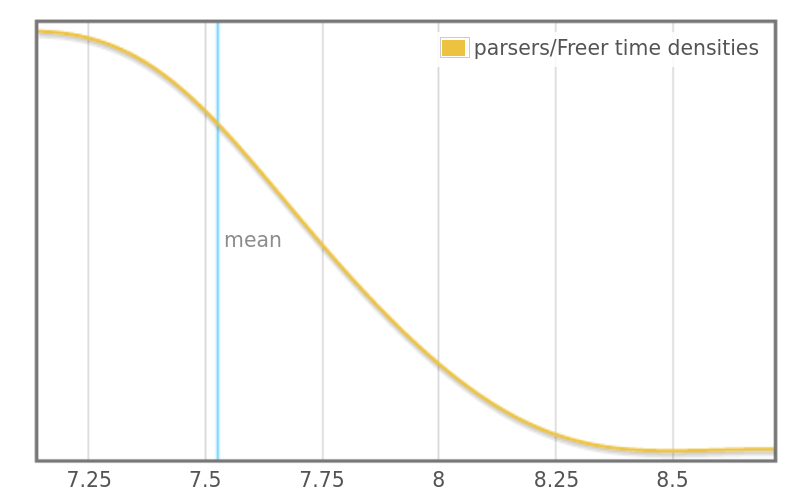
\includegraphics[scale=0.4]{images/freer.png}
      \caption{Monad transformers parsers benchmark}
      \label{mtlParserBench}
      \end{figure}

      The benchmarking was performed for a parser of a Markdown"/like language
      implemented using this library. The benchmarked action was parsing of a
      file of size about 3 kilobytes. The benchmark, together with the source code
      of the library and the parser may be found in the library's GitHub
      repository~\cite{extEffParsers}.

      This benchmark shows extensible effects to work slower in comparison to the monad transformers based implementation (see chapter~\ref{cpt-monads:parsers-bench}).

      \subsection{Conclusion}

      Extensible effects are an embedding of algebraic effects and handlers in Haskell,
      thus the sketched parser combinators library has a lot in common with the one
      implemented in Frank (see previous section). However, as far as Extensible
      Effects are implemented on top of free monads, programmer must adopt the monadic
      style for definition of effectful computations and parsers implementation
      become a bit more wordy than in Frank.


\chapter{Functional programming and computational effects control at scale}
~\label{cpt-effects}

This chapter presents and discusses ``Student's Big Brother'' --- a distributed
system to support study workflow in a programming class. It was designed to help
teachers to distribute their attention to all students uniformly. The system consists
of client daemons, watching students activity and sending their source code to a server (over HTTP),
for storage, processing and displaying in teacher web"/interface.
The source code is freely available on GitHub~\cite{sbbRepo}.

The system is mostly implemented using Haskell programming language and the implementation
extensively uses monad transformers and algebraic effects --- the concepts discussed previously
in this thesis --- to structure the necessary side"/effects and separate the effectful
functionality from the pure code.

The rest of the chapter is structured as follows: the first section gives a short
note on motivation for the system's creation; the second section abstractly describes
the system's architecture; the third section focuses on implementation details:
configuration files, integration and deployment and benefits of the use of functional
programming; the last section reports the system usage in real"/life teaching.

\section{Motivation}

It is unfortunate, but most undergraduate students hesitate to ask questions during
programming practice sessions. Usually, the instructing teacher is fighting
students' shyness by walking around the room, observing students and trying to
determine whether the particular student is succeeding or not. But due to the
limited time of the sessions and the fact that there is only one instructor per
10"/15 students, the described procedure is quite inefficient. To approach the
problem, we propose to build a monitoring system for students activities during
programming classes. This system should have features of basic
version control and of displaying the students' source code in a lightweight
web"/interface for the instructor to be able to observe the activity of every
student in real"/time.

The primary purpose of the system is to distribute teachers attention between
all the active students uniformly and to help the teacher to determine which one
needs an assistance but hesitates to ask for it.

\section{System's architecture}

\usetikzlibrary{shapes, arrows, calc, positioning}

\tikzset{
    module/.style={
           rectangle,
           rounded corners,
           draw=black, very thick,
           minimum height=2em,
           inner sep=2pt,
           text centered,
           },
}


\begin{tikzpicture}[->,>=stealth']

 \node[ellipse, draw=black, very thick] (TEACHER)
 {%
  \textbf{Teacher}
 };

 \node[module,
  yshift=-1cm,
  text width=2cm,
  below of=TEACHER] (UI)
 {%
  \textbf{Web UI}
 };

 \node[module,
  text width=3cm,
  yshift=-1cm,
  below of=UI] (SERVER)
 {%
  \textbf{Server}\\
 };

 \node[module,
  below of=SERVER,
  yshift=-1cm,
  xshift=-4cm,
  anchor=center,
  text width=3cm] (DAEMON_1)
 {%
  \textbf{Daemon}
 };

 \node[module,
  right of=DAEMON_1,
  xshift=3cm,
  text width=3cm] (DAEMON_2)
 {%
  \textbf{Daemon}
 };

 \node[module,
  right of=DAEMON_2,
  xshift=2cm,
  draw=none,
  text width=1cm] (HIDDEN_DAEMONS)
 {%
  \textbf{...}
 };

  \node[module,
  right of=HIDDEN_DAEMONS,
  xshift=2cm,
  text width=3cm] (DAEMON_3)
 {%
  \textbf{Daemon}
 };

 \node[module,
  right of=SERVER,
  xshift=3cm,
  text width=2cm] (DB)
 {%
  \textbf{DB}
 };

 \node[ellipse, draw=black, very thick,
       below of=DAEMON_1,
       yshift=-1cm, ] (STUDENT_1)
 {%
  \textbf{Student}
 };

  \node[ellipse, draw=black, very thick,
       below of=DAEMON_2,
       yshift=-1cm, ] (STUDENT_2)
 {%
  \textbf{Student}
 };

  \node[ellipse,
       below of=HIDDEN_DAEMONS,
       yshift=-1cm, ] (HIDDNE_STUDENT)
 {%
  \textbf{...}
 };

  \node[ellipse, draw=black, very thick,
       below of=DAEMON_3,
       yshift=-1cm, ] (STUDENT_3)
 {%
  \textbf{Student}
 };

 \path (DAEMON_1) edge (SERVER);
 \path (DAEMON_2) edge (SERVER);
 \path (DAEMON_3) edge (SERVER);

 \path (SERVER) edge (DB);
 \path (DB) edge (SERVER);

 \path (SERVER) edge (UI);
 \path (UI) edge (SERVER);

 \path (TEACHER) edge[dashed] (UI);

 \path (STUDENT_1) edge[dashed] (DAEMON_1);
 \path (STUDENT_2) edge[dashed] (DAEMON_2);
 \path (STUDENT_3) edge[dashed] (DAEMON_3);

\end{tikzpicture}

The system consists of three software components: the server, the client daemon and the
teacher's web user interface (UI). The communication between all participants is performed
over HTTP using JSON"/formatted messages.

The rest of this section gives a more detailed account of the role of every component.

\subsection{Daemon: data collection agent}

The client daemon is a data collection agent. It is designed to run silently on
a student's computer, observe student's activity and report it to a server.

The daemon's operation protocol is simple: it runs on a student's computer,
watches the working directory for changes in source code files and regularly sends
these changes to the application server for storage and distribution.

\subsection{Server: data keeper and distributor}

The server's role is to be the central authority for the daemons: collect the files
the send, store them in a database and give them to the web UI on demand.

The server's code is essentially a CRUD"/service~\cite{Martin:1983:MDB:538746} ---
it implements creation, removing, updating and deletion procedures of the considered
entities --- source code files  --- and maps these operations onto database procedures.

\subsection{Web UI: data presenter}

The web UI conveys the information about current state of students works to the teacher.
It keeps up with the present state of server's database and provides a minimalistic
interface to browse the files of every student separately.

\section{Implementation details}

The server and the client daemon are implemented with Haskell programming language
and employ Haskell's type system to enforce safety and correctness of operation
and communication. The teacher's web application is built with standard web stack:
HTML, CSS and JavaScript.

\subsection{Type"/safe communication: sharing types between client and server}

\subsection{Extensible effects at daemon's service}

\section{Exploitation experience report}

The experiment of integration of the developed system into the teaching workflow
of an undergraduate programming course in I.~I.~Vorovich institute of mathematics,
mechanics and computer science was successful. A teacher who has been leading the
class reported the system to be reliable and the user experience to be satisfying.
It was also reported that students had been showing more effort to complete the
tasks and their hesitation for asking questions have been significantly reduced.


\Conc

This thesis contributes to the development of approaches to effectful computation.
Implementations of three parser combinators libraries based on three
effectful computation frameworks are presented: one based on Haskell
monad transformers~\cite{mdParse};
another implemented with extensible effects~\cite{extEffParsers}~
--- an embedding of algebraic effects
and effects handlers into Haskell; and a third one is a prototype implementation
of a parser combinators library in Frank~\cite{frankoparsec}~---
an experimental programming language
with native support for programming with algebraic effects and effects handlers.

The developed libraries demonstrate advantages and disadvantages of the considered
approaches. The thesis also gives an account to performance benchmarking of the monad
transformers and extensible effects based libraries.

While building the prototype parsing library in Frank, we found out the limit of
expressibility of algebraic effects in Frank: currently, it is impossible to
declare effects which would have commands yielding results of different types;
thus making impossible to implement full"/fledged parser as a monolithic effect.
A possible future work may include an extension of Frank's effect system to support
existential quantification or GART"/like syntax for commands of effect interfaces.

The last chapter of the thesis describes an application of functional programming
language with side"/effects control to development of real"/life software. We
present the architecture and explain the implementation details of a distributed
system for real"/time student activity monitoring
``Students Big Brother'''~\cite{sbbRepo}. We exploits the Haskell's type and effect
systems to make the implementation reliable and maintainable. The server"/side share
the domain types with the client code thus making it impossible fir them to diverge.
The server"/side effects is structured with monad transformers and the data collection
daemon code uses extensible effects. We report our experience on how advanced type system
features may improve the maintainability of a code base, make a development process
more structured, and, as a result, lead to a reliable software.



% Печать списка литературы (библиографии)
\printbibliography[%{}
    heading=bibintoc%
    ,title=Bibliography % если хочется это слово
]
% Файл со списком литературы: biblio.bib
% Подробно по оформлению библиографии:
% см. документацию к пакету biblatex-gost
% http://ctan.mirrorcatalogs.com/macros/latex/exptl/biblatex-contrib/biblatex-gost/doc/biblatex-gost.pdf
% и огромное количество примеров там же:
% http://mirror.macomnet.net/pub/CTAN/macros/latex/contrib/biblatex-contrib/biblatex-gost/doc/biblatex-gost-examples.pdf

\end{document}
